
\section{Seznam funkčních požadavků}\label{sec:seznamFunkčníchPožadavků}

Před začátkem návrhu každé aplikace je důležité definovat funkční požadavky.
Funkční požadavky slouží k vymezení toho, co má aplikace umět a co již umět nemusí.
Jednotlivé funkční požadavky jsou dále rozšířeny uživatelskými případy (viz sekce~\ref{sec:uzivatelskePripady}), které definují použití jednotlivých funkcí aplikace.

\begin{figure}[ht!]
    \centering
    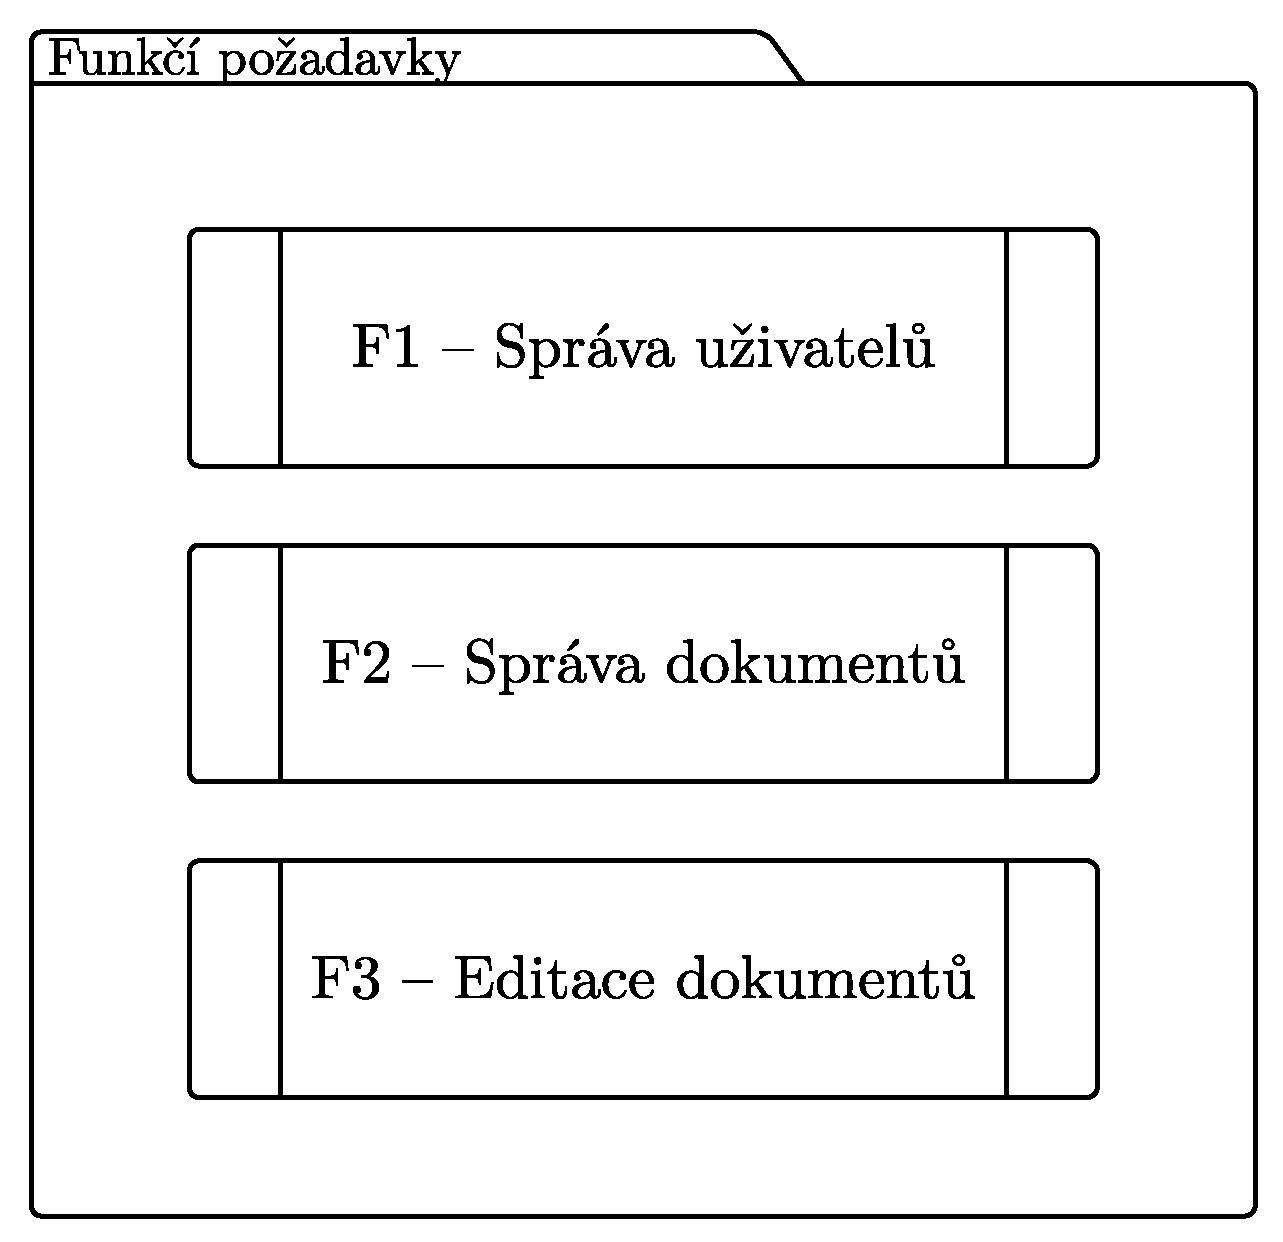
\includegraphics[width=0.6\textwidth]{partials/analyza/funkcniPozadavky.pdf}
    \caption{Diagram funkčních požadavků}\label{fig:funkciPozadavky}
\end{figure}

\paragraph{F1 -- Správa uživatelů}

Tento požadavek představuje možnost vytvoření uživatelského účtu a jeho používání.
Každý uživatel bude mít uživatelské jméno, které je pro každého uživatele unikátní a slouží jako jeho identifikátor mezi ostatními uživateli.
Uživatel si může své přihlašovací i jiné údaje po přihlášení kdykoliv změnit.

\paragraph{F2 -- Správa dokumentů}

Přihlášený uživatel si může nechat zobrazit vytvořené dokumenty, vytvořený dokument smazat, či vytvořit dokument nový.
Dokumenty jsou vázány na uživatele, který ho vytvořil (dále jen majitel dokumentu), a dokument nelze mezi uživateli přesouvat.

\paragraph{F3 -- Editace dokumentů}

Uživatelé mohou upravovat jednotlivé dokumenty ve skutečném čase spolu s ostatními uživateli.
U každého dokumentu bude k dispozici komunikační vlákno, kde mohou uživatelé, kteří dokument upravují, komunikovat mezi sebou.
Uživatelé mohou pro přístup k dokumentu použít jeho veřejný odkaz nebo mohou být k dokumentu pozváni jednotlivě.
Jednotlivý uživatelé, krom majitele, mohou mít možnosti editace dokumentu omezeny pomocí nastavení práv dokumentu.
